\documentclass{sig-alternate-sigmod09}

\usepackage[bookmarks=true,pdfborder= 0 0 0]{hyperref}

\usepackage{tikz}
\usetikzlibrary{calc,trees,positioning,arrows,chains,shapes.geometric,%
  decorations.pathreplacing,decorations.pathmorphing,shapes,%
  matrix,shapes.symbols,plotmarks,decorations.markings,shadows}

\DeclareMathOperator{\atantwo}{atan2}

\hypersetup{
pdfauthor={Patrick Brosi},
pdfkeywords=,
pdftitle={A Simple Approximation Algorithm for Metro Map Drawing},
pdfsubject={},
pdfcreator={},
pdfproducer={}
}

\begin{document}
\title{An Approximation Algorithm for Drawing Metro Maps}

\numberofauthors{1}
%\author{Patrick Brosi\\\affaddr{University of Freiburg}\\\affaddr{Chair of Algorithms and Data Structures}}

\maketitle

\section{Abstract}

We investigate a novel approximative approach to octilinear Metro Map drawing. Contrary to previous work, which usually relied on either local or global optimization techniques, we state the task as a (greedy) iterative shortest-path problem on a specially crafted octilinear grid graph, whose edge weights are updated after each iteration. While our results are not perfect, they come surprisingly close to previous work which used Integer Linear Programming to find a globally optimal solution. We state the basic idea of our approach, give some heuristics to improve the final result and evaluate our method on 5 cities around the world. The resulting maps are rendered using previous work by us and are publicly accessible at http://bla.blubb. 

\section{Problem definition}

\section{Related Work}

Survey Nöllenburg http://i11www.iti.kit.edu/extra/publications/n-asamm-14.pdf
Survey Wolff http://www1.pub.informatik.uni-wuerzburg.de/pub/wolff/pub/w-dsms-07.pdf
Hong et al., force-based approach
Stott's PhD



\section{Map Generation}

\subsection{Octilinear Grid Graph}

We want to construct a graph $G$ on which every path is octilinear. The graph in Fig.~\ref{FIG:gridgraph} trivially guarantees this. Additionally, we want the total cost for a path from some node $a$ to another node $b$ to also reflect the total number of turns on this path. The cost of a turn should be weighted by the degree of this turn - either $135^{\circ}$, $90^{\circ}$ or $45^{\circ}$. We call these penalties $p_{135}$, $p_{90}$ and $p_{45}$. A straight pass through a node should go unpunished, that is, $p_{180} = 0$. Since we aim for a ``smooth'' path through $G$ we want to favor obtuse angles and require $p_{180} < p_{135} < p_{90} < p_{45}$.

The cost of any edge in Fig.~\ref{FIG:gridgraph}, left then depends on the edge we came from. We model this by adding 8 \emph{port} nodes $v_i^0 ... v_i^7$ to every node $v_i$. Each port corresponds to an outgoing direction - $v_i^0$ is the ``north'', $v_i^1$ is the ``south-west'' port and so on. Each port is connected with a direct edge $e_i^0 ... e_i^7$ and the cost for each of these edges is set to ``infinity minus one'' - that is, the cost has to bigger than the maximum possible cost of any other edge. This ensures that these edges are only used if we actually want to arrive in $v_i$. For passing through $v_i$, we connect each port with its neighbor at $90^{\circ}$ $135^{\circ}$ and $180^{\circ}$ (Fig.~\ref{FIG:port}, middle). It will become apparent later on why we skip $45^{\circ}$ edges here.

A $180^{\circ}$ pass through $v_i$ can now take the direct edge connecting each port $v_i^k$ with its $180^{\circ}$ neighbor $v_i^{(k + 4) \mod 8}$ (Fig.~\ref{FIG:paths}, 1). Equally, a $90^{\circ}$ degree turn in $v_i$, coming from $v_i^k$ can take the edge to $v_i^{(k + 2) \mod 8}$ (Fig.~\ref{FIG:paths}, 2) and so on.

As both a $45^{\circ}$ turn and a $90^{\circ}$ turn can be simulated by two (or more) cheaper turns, special care has to be applied to the modelling of the actual edge costs. A $45^{\circ}$ turn can be simulated by first passing $v_i$ on a $180^{\circ}$ edge, and then again on a $135^{\circ}$ edge (Fig.~\ref{FIG:paths}, 3). As $p_{180} < p_{135} < p_{45}$, this path may be cheaper than $p_{45}$. Similarily, a $90^{\circ}$ degree turn can be simulated by two cheaper $135^{\circ}$ edges (Fig.~\ref{FIG:paths}, 4).

We call the actual edge costs for the 4 classes of port-to-port edges $c_0$, $c_{135}$, $c_{90}$ and $c_{45}$. To prevent the shortcuts described above, we make use of the fact that the absolute costs of these edges are irrelevant - since they are modeled the same in every node in $G$ and a path passing through (not going to) $v$ has to take one of them, we just have to make sure that the relative costs reflect the penalties we want to apply to the different angles, that is, $c_{135} - c_{180} = p_{135}$, $c_{90} - c_{180} = p_{90} = p_{135} + (c_{90}-c_{135})$ and so on. 

\begin{figure*}[h]
  \centering
	$\vcenter{\hbox{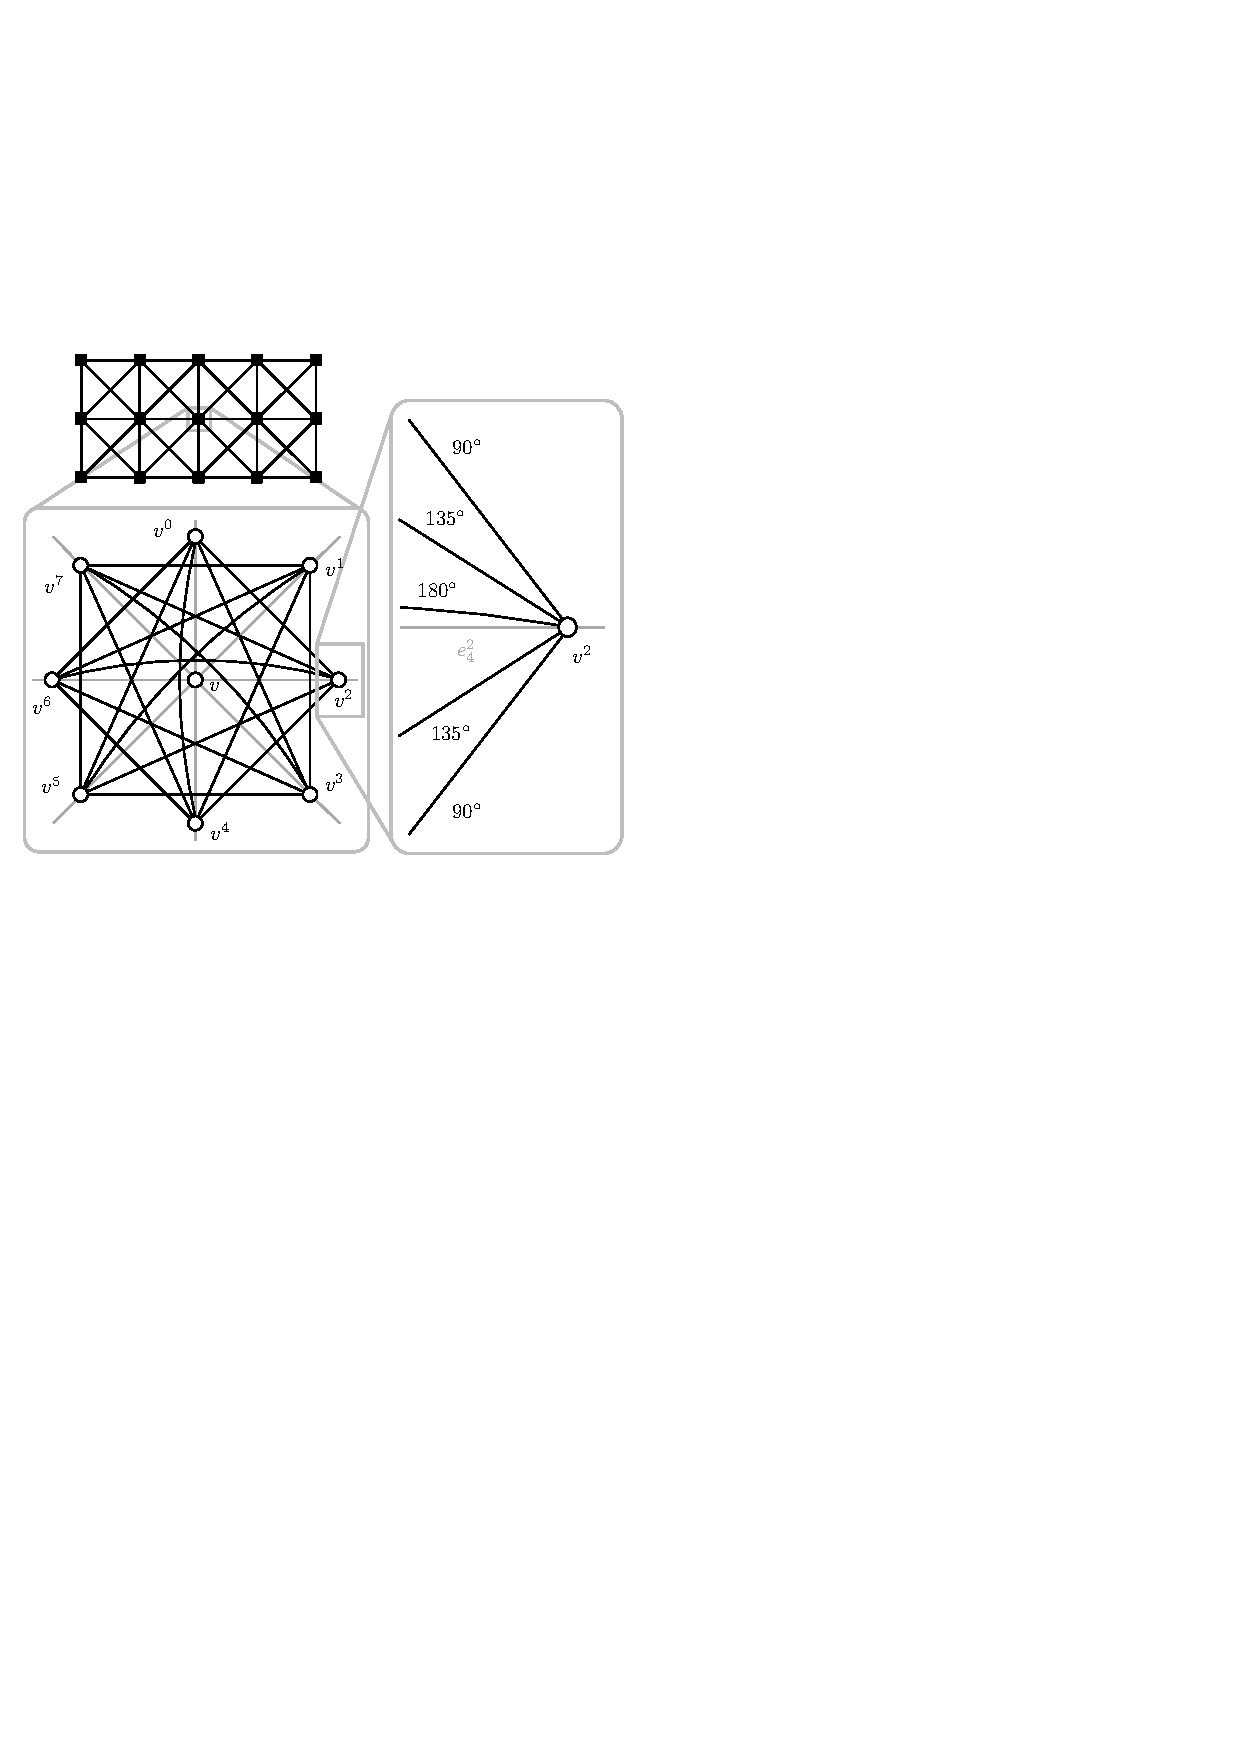
\includegraphics[width=0.85\textwidth]{figures/node.pdf}}}$
	\caption{A $3\times3$ grid graph. Each node $v_i$ has 8 ports $v_i^0 ... v_i^7$ which are connected to $v_i$ by a direct edge. Each port is additionally connected to its $180^{\circ}$, $135^{\circ}$ and $35^{\circ}$ neighbor ports.}
	\label{FIG:gridgraph}
\end{figure*}

Following this insight, we introduce a constant $a \geq 0$ and calculate the inter-port edge costs as follows:
\begin{align}
c_{180} &= a \\
c_{135} &= a + p_{135} \\
c_{90} &= a + p_{90} \\
c_{45} &= a + p_{45}.
\end{align}

We choose $a$ in a way such that the following constraints are fullfilled:
\begin{align}
2a + p_{135} &\geq a + p_{90} \label{CONSTRS:sim90}\\
2a + p_{135} + p_{90} &\geq a + p_{45}\label{CONSTRS:sim45}.
\end{align}
(\ref{CONSTRS:sim90}) ensures that simulating a $90^{\circ}$ pass with two $135^{\circ}$ passes is never cheaper than $c_{90}$. (\ref{CONSTRS:sim45}) ensures that simulating a $45^{\circ}$ pass with a $135^{\circ}$ pass and a $180^{\circ}$ pass is never cheaper than $c_{90}$.

(\ref{CONSTRS:sim45}) and (\ref{CONSTRS:sim90}) are fullfilled for $a = p_{45} - p_{135} \geq 0$, leading to the following edge costs in $G$:

\begin{align}
c_{180} &= p_{45} - p_{135} \\
c_{135} &= p_{45} \\
c_{90} &= c_{180} + p_{90} \\
c_{45} &= 2p_{45} - p_{135} = c_{180} + c_{135}.
\end{align}

We can thus do without an explicit edge for $45^{\circ}$ turns, as it can always be exactly simulated.


\begin{figure*}
  \centering
	$\vcenter{\hbox{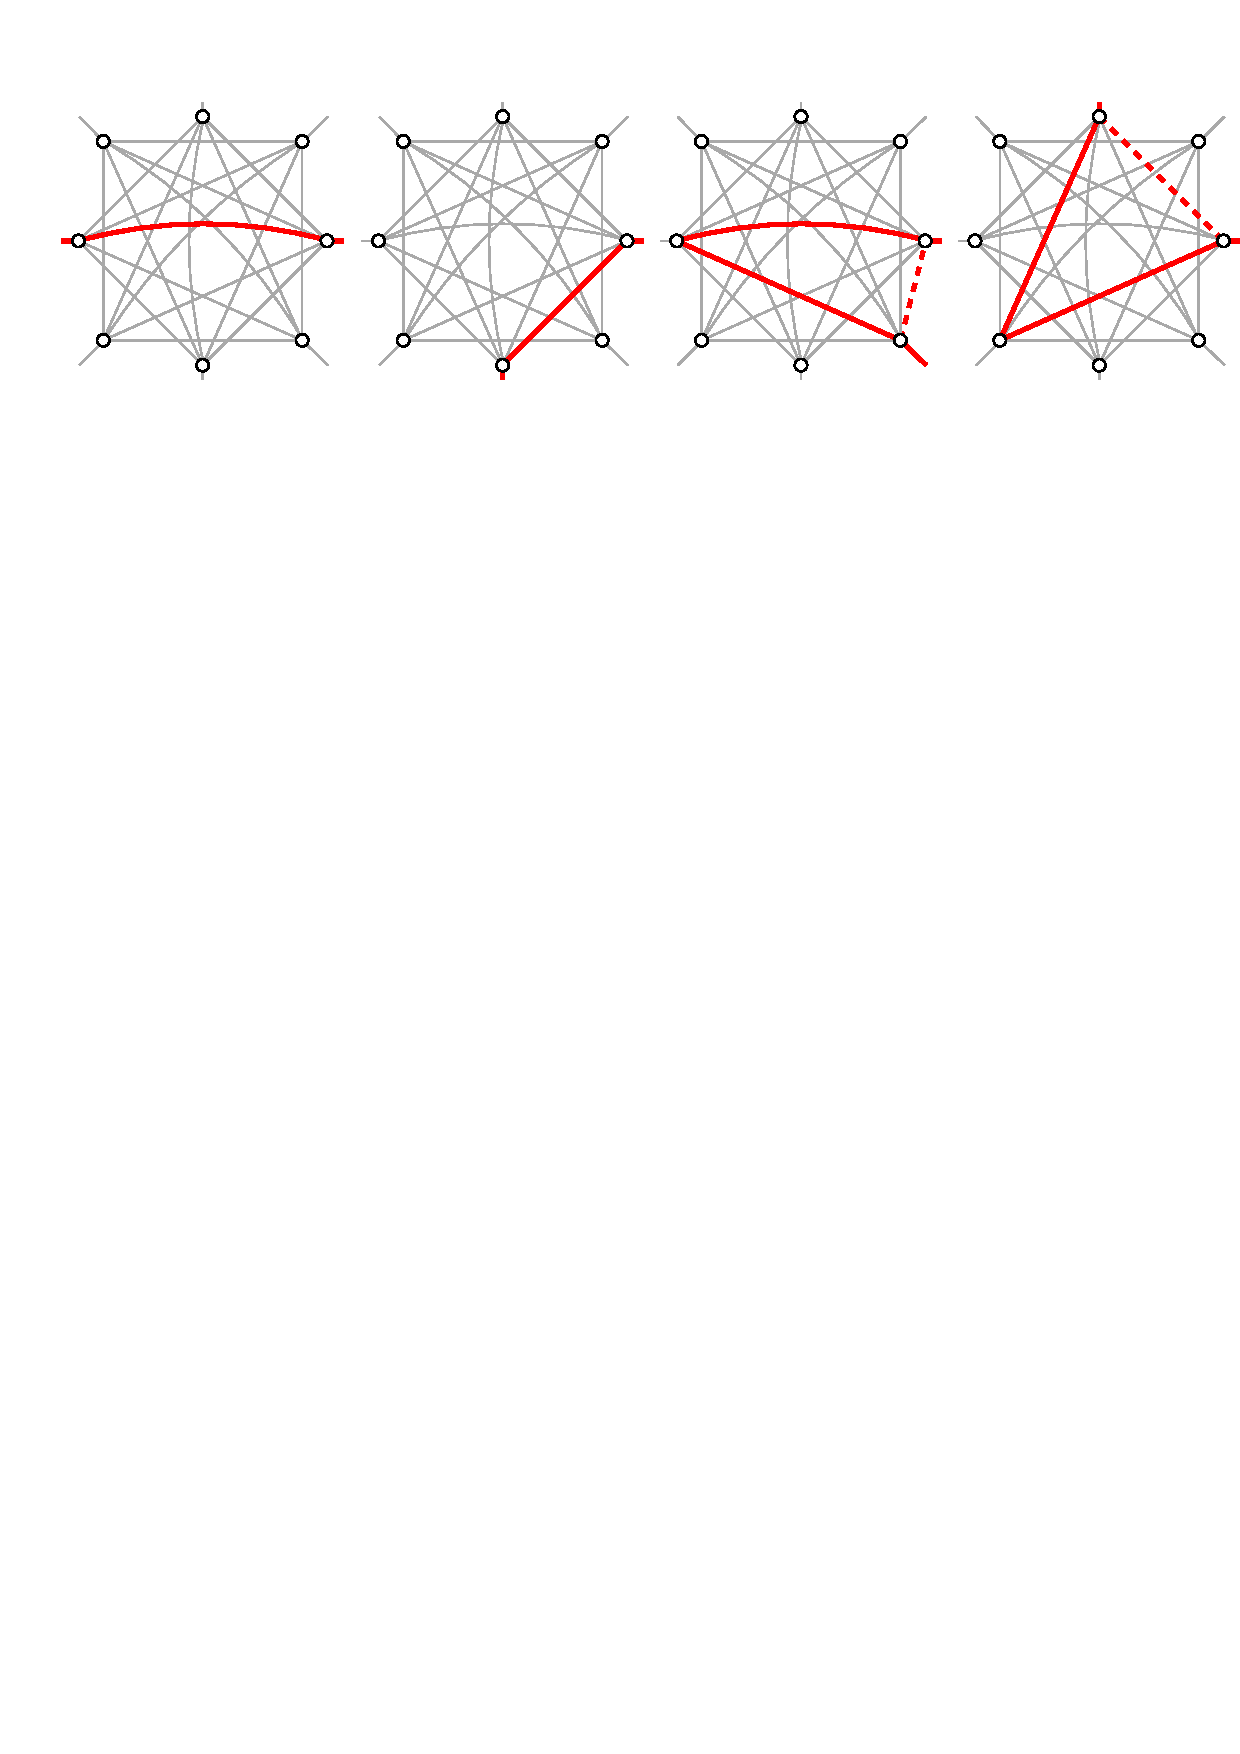
\includegraphics[width=0.9\textwidth]{figures/paths.pdf}}}$
	\caption{1. A $180^{\circ}$ pass through a node $v$. 2. A $90^{\circ}$ pass through $v$. 3. A $45^{\circ}$ pass through $v$ simulated by a $180^{\circ}$ and $135^{\circ}$ pass. 4. A $90^{\circ}$ pass through $v$ simulated by two $135^{\circ}$ passes. }
	\label{FIG:paths}
\end{figure*}


\subsection{Input Ordering}

\section{Preserving Topology}

\section{Evaluation}

\subsection{Penalty Experiments}

\section{Conclusion}

\balancecolumns
\end{document}
